%
% File: chap02.tex
% Author:
% Description: Background
%
\chapter{Background}
\label{chap:background}

% Description

\section{Relative Work}
\label{sec:relative-work}


% SDG Goal 3

In many hospitals, patients need to wait for a long time just to have a short consultation with a doctor. This can be exhausting, especially for people who are already sick. In some places like the countryside, the problem is worse because there are not enough doctors or clinics \cite{ilo_ruralgap}. Some people need to travel very far to get help, which is hard for old people or people with long-term illness.

During COVID-19, many doctors started using phone or video to talk to patients. In the UK, it went from 15\% to 48\% in just a few weeks \cite{nuffield_gp}. It helped people talk to doctors from home and also saved time.

Our Smart Hospital system also uses phone and video consultations. We also have Health QA, where people can ask simple health questions and get advice more easily. These help people who live far away or cannot go outside, and they also make the waiting time in hospitals shorter.

Our system supports the United Nations’ SDG Goal 3, which is about helping people stay healthy and live well \cite{un_sdg3}. Among all the targets, Goal 3.8 and Goal 3.4 are especially important to our project. Goal 3.8 is about giving basic and affordable health services to everyone. Goal 3.4 is about helping people with long-term sickness, like heart disease or mental problems. Our system lets them contact doctors or get advice online more easily, so they can get help earlier before the problem becomes worse.

\section{Existing Solutions}
\label{sec:existing-solutions}

% write soultion

\subsection{Teladoc Health}
% 內容...
Teladoc Health is a popular online medical platform\cite{teladocwebsite} that offers services like video calls with doctors and support for mental health. It is used in many countries and is helpful for people who find it hard to go to a hospital. But one problem is that it’s not fully connected to real hospitals. This means doctors on Teladoc often can’t see a patient’s full medical records from other clinics or hospitals. As a result, some information might be missing, which can make it harder to give the right diagnosis or follow-up care.


\begin{figure}[htbp]
    \centering
    \begin{minipage}[b]{0.47\textwidth}
        \centering
        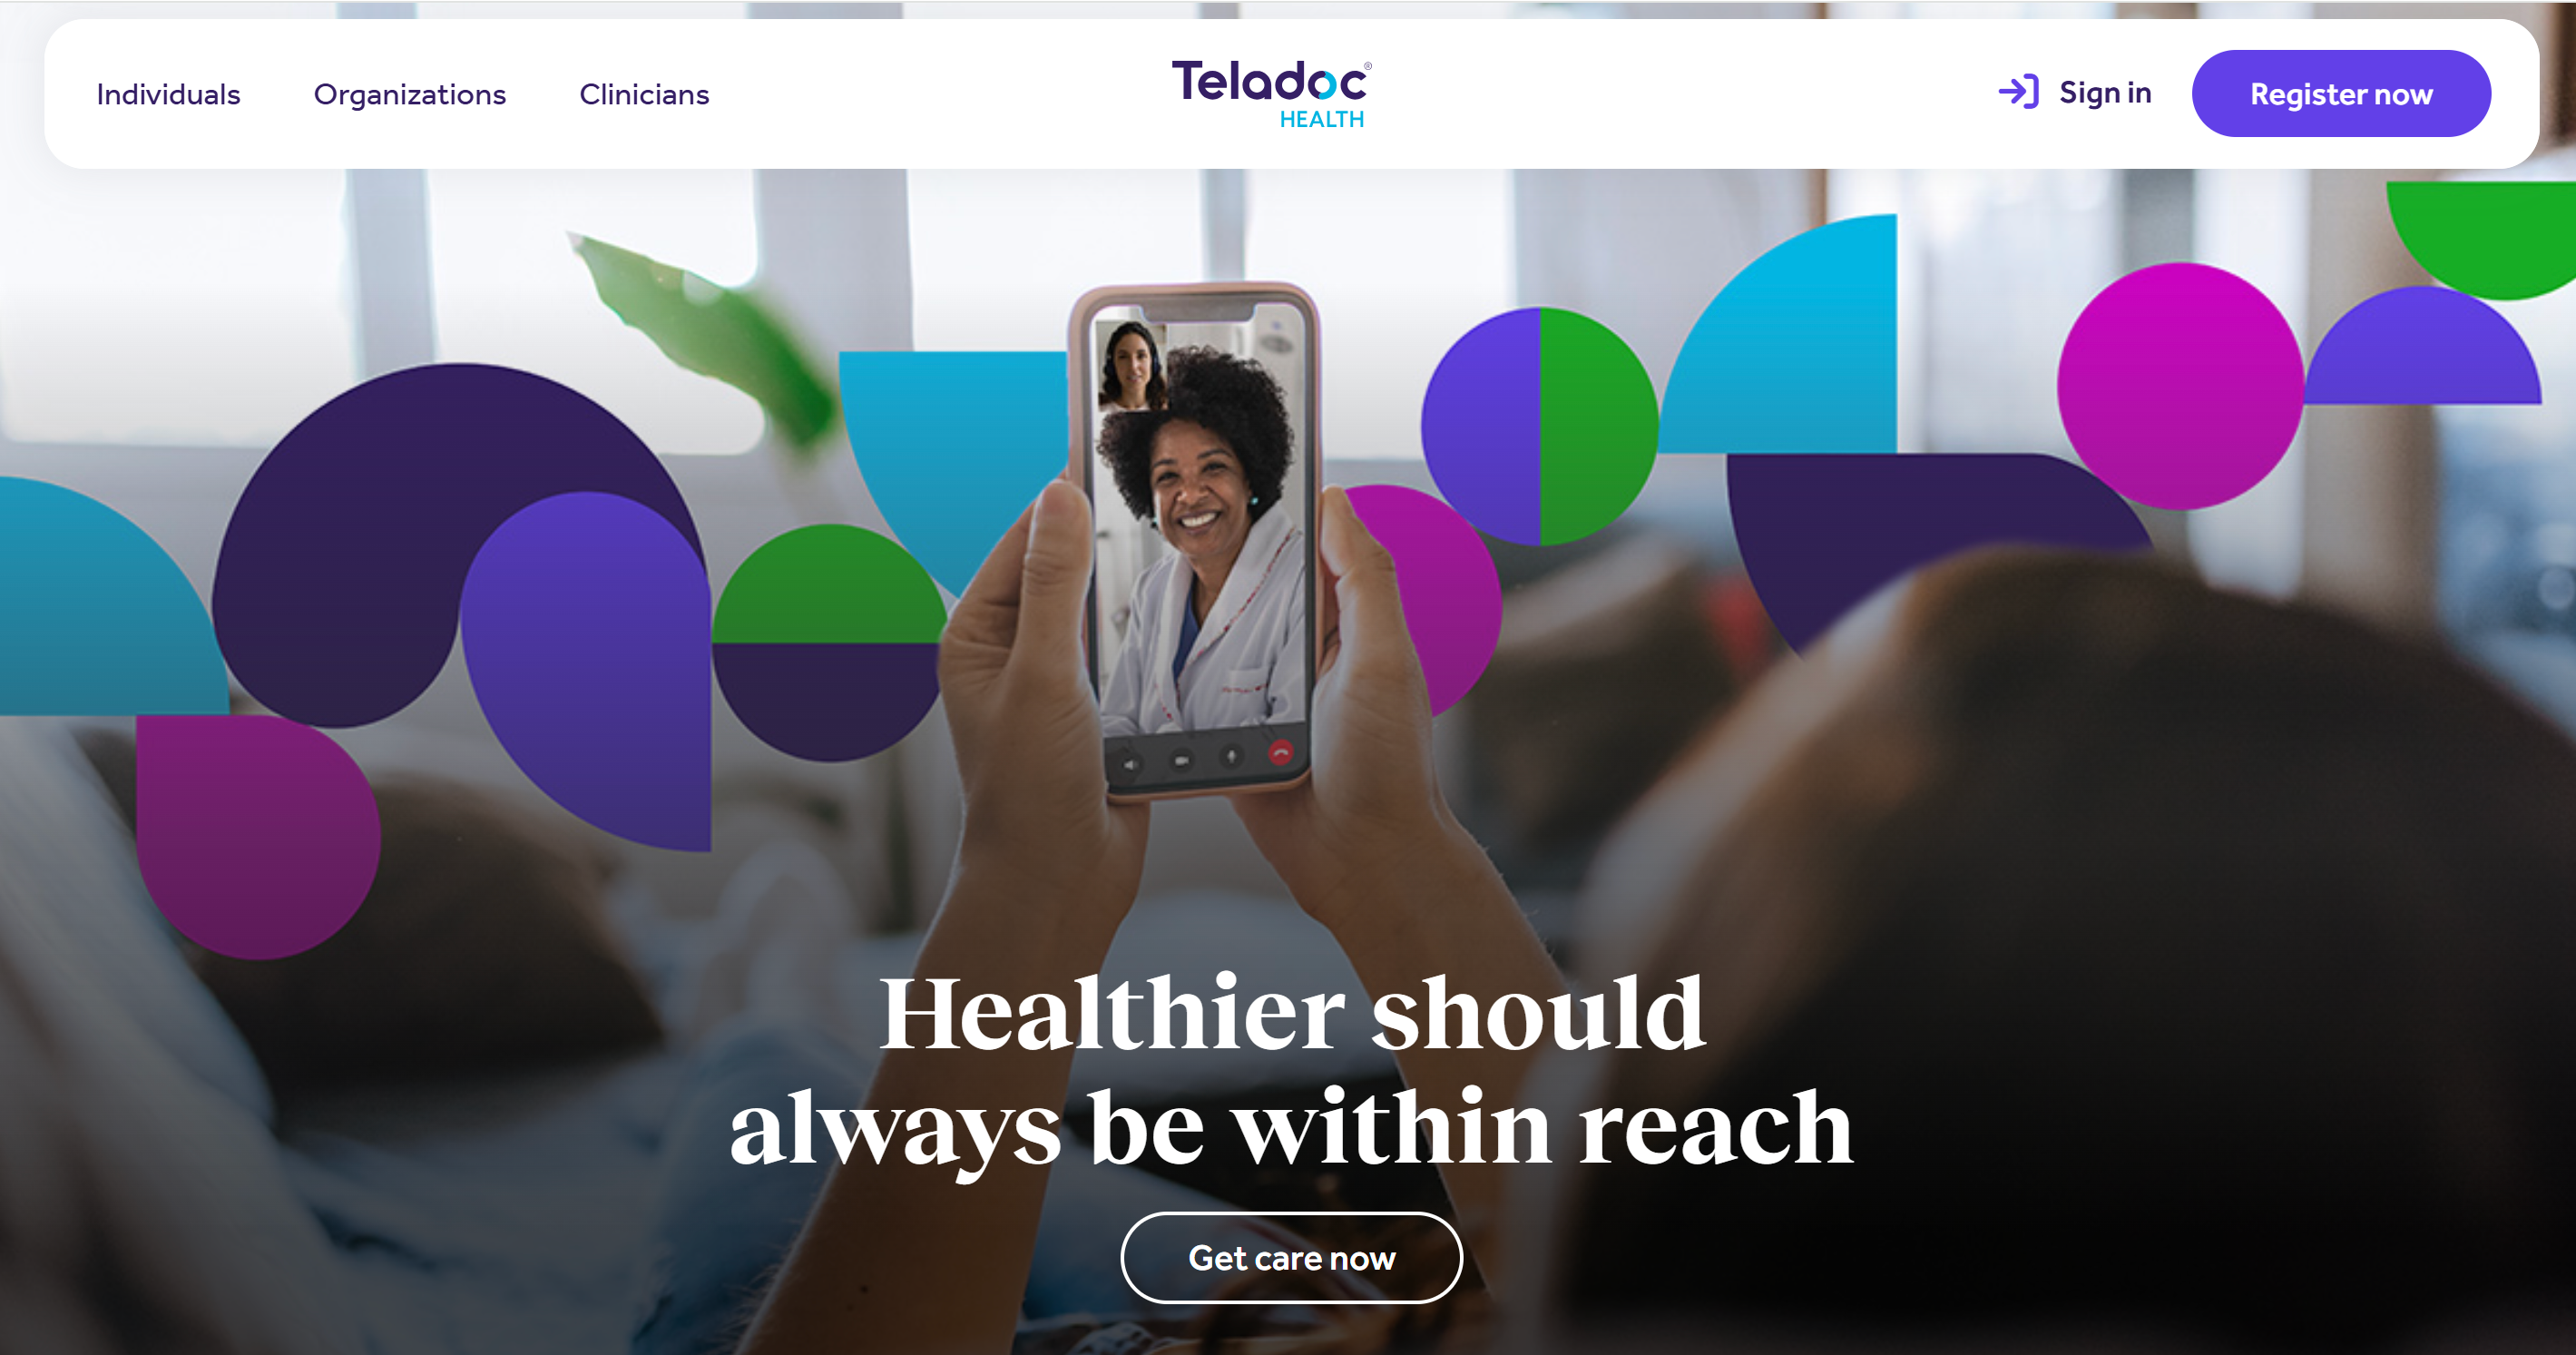
\includegraphics[width=\textwidth]{../../images/telodocHome.png}
        \caption{Homepage of Teladoc Health.}
        \label{fig:teladoc-home}
    \end{minipage}
    \hfill
    \begin{minipage}[b]{0.47\textwidth}
        \centering
        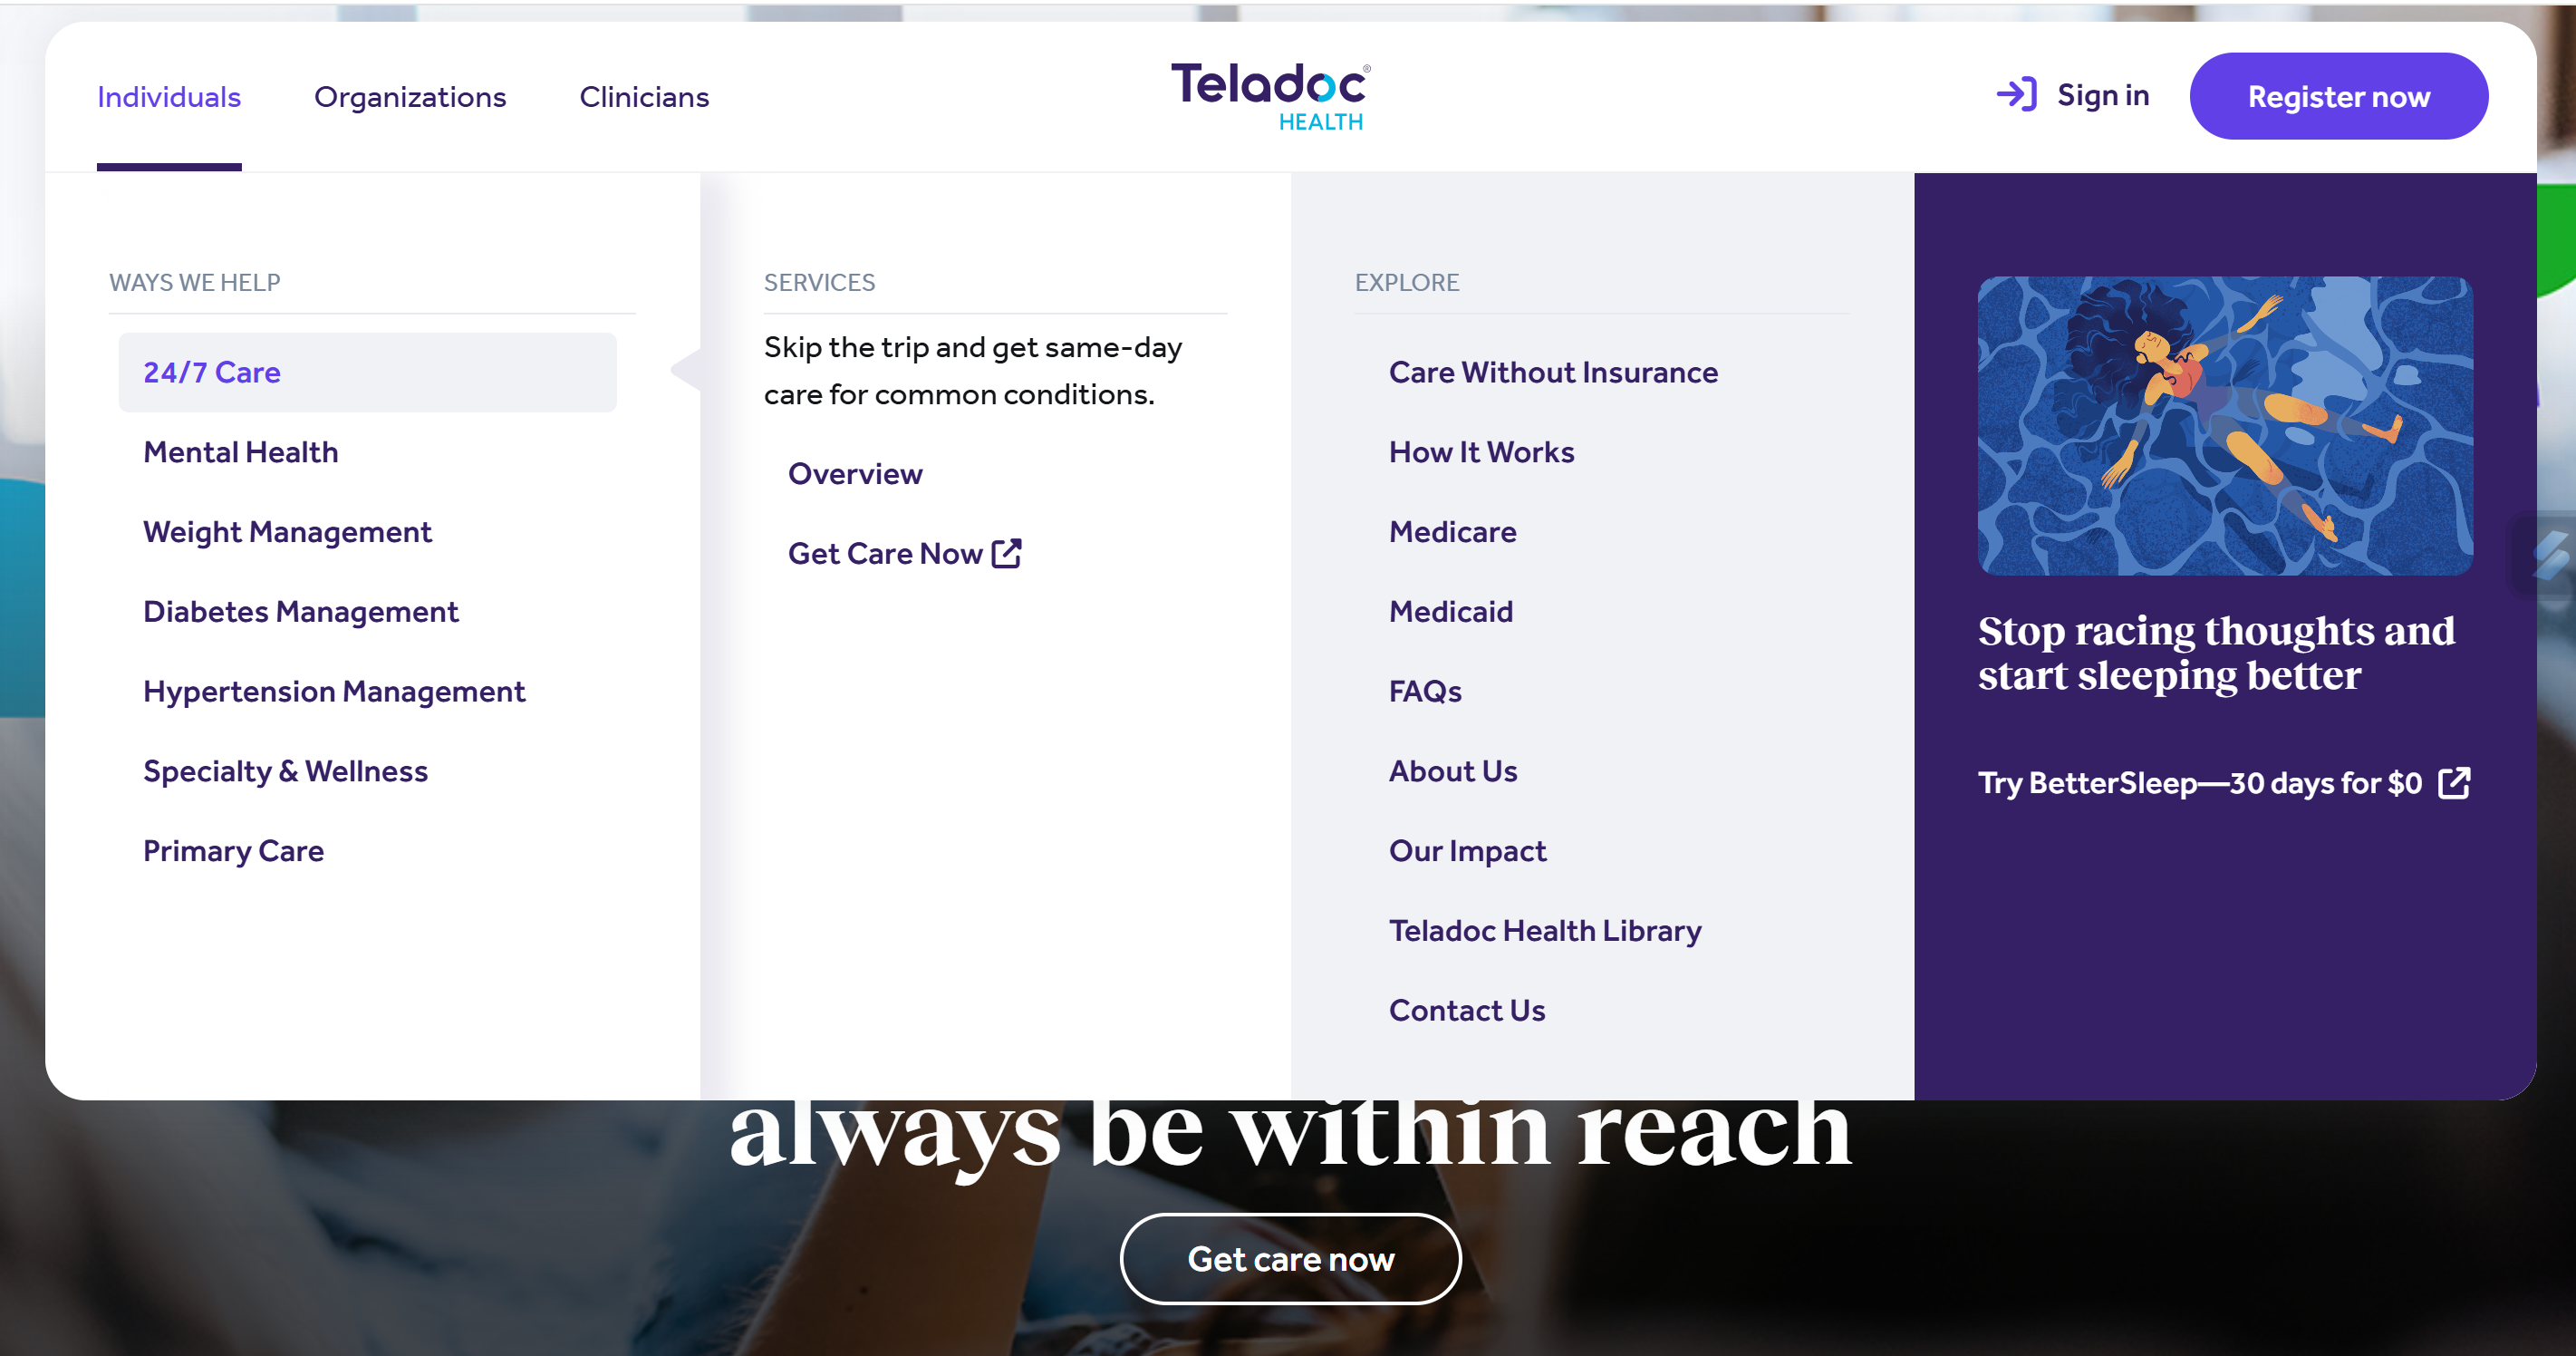
\includegraphics[width=\textwidth]{../../images/telodocServices.png}
        \caption{Service menu of Teladoc Health.}
        \label{fig:teladoc-services}
    \end{minipage}
\end{figure}

\subsection{LINE Hospital Services}
In Taiwan, many hospitals have their own official LINE accounts to provide online services. Patients can add the hospital’s LINE to access booking and other basic functions. It is very easy to use, since most people in Taiwan already use LINE in their daily life. This makes it a common way for hospitals to offer simple medical services without asking people to download another app.

\noindent
\begin{figure}[htbp]
    \centering
    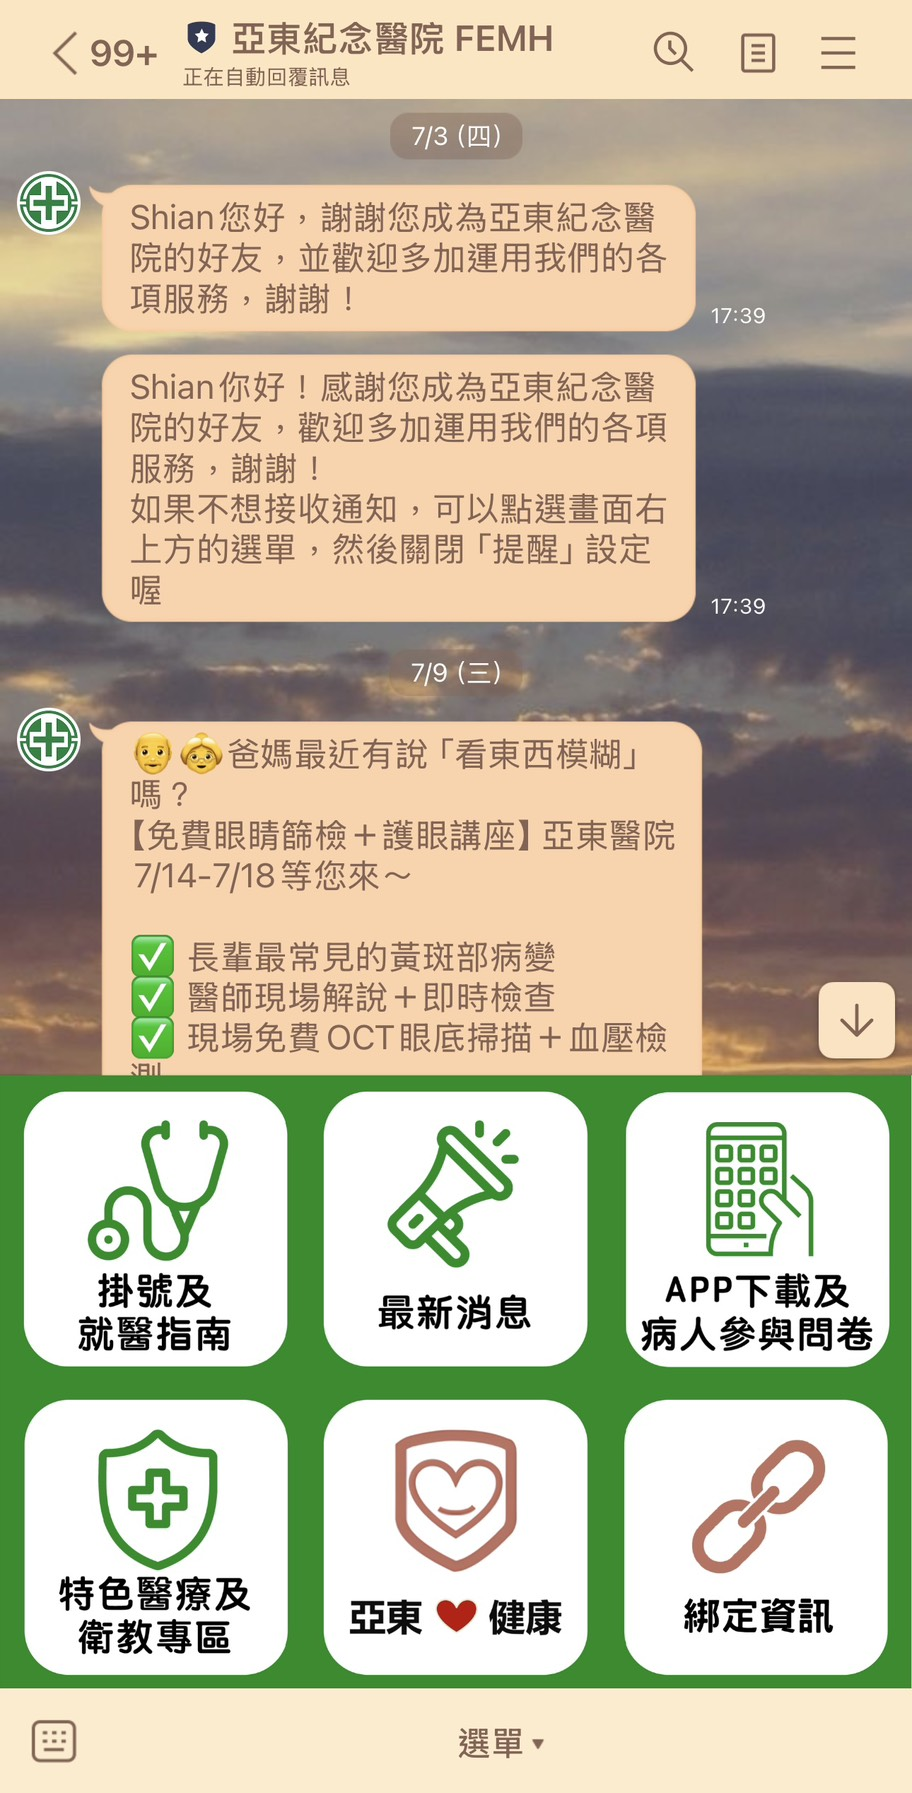
\includegraphics[width=0.2\textwidth]{../../images/line.jpg}
    \caption{Screenshot of LINE services from Far Eastern Memorial Hospital, showing options like booking, announcements, and personal info links~\cite{femhline}.}
    \label{fig:line-service}
\end{figure}
\noindent

These features are quite easy to use. However, each hospital has its own design and menu. Some functions even open in separate websites. There is no unified system, so it can be confusing for some patients, especially older people or those not familiar with technology.



\clearpage


\clearpage
\section{Requirements}
\label{sec:requirements}

The system is designed as a web-based platform for doctors, nurses, and patients to facilitate efficient clinical workflows and improve access to healthcare services. The main objective is to allow healthcare staff to manage patient information, record essential clinical data, and provide consultations remotely, thereby reducing unnecessary hospital visits. Patients are also supported with features to access their health records and receive guidance without needing to attend the hospital in person.

To ensure a functional and effective experience for hospital staff and patients, the system was designed to support a core set of features. These include secure user login and authentication for doctors, nurses, and patients; the ability to record patient vitals and view historical data trends; and an interface for remote consultation to minimise unnecessary hospital visits.

Drawing on the team’s previous experience with similar healthcare platforms, including the Virtual Hospital Africa system, we referenced their approach as a conceptual foundation while adapting the design to our own project scope and requirements.

The system is initially populated with pre-existing mock patient data to facilitate testing and demonstration. In addition to these accounts, the platform supports new patient registration, enabling patients to create their own accounts and access the same core features, including secure login, health query submission, and medical record downloads.

Non-functional requirements include secure authentication with role-based access control, ensuring that only authorised users can access or modify clinical records. The system is designed for stable operation with fast response times to support real-time clinical workflows. In addition, the user interface is kept clear and intuitive to reduce training time for hospital staff. These system capabilities are closely aligned with the user stories
presented below.

\vspace{1em}
\begin{table}[H]
\centering
\renewcommand{\arraystretch}{1.4}
\begin{tabular}{|p{2cm}|p{5.2cm}|p{5.2cm}|p{2cm}|}
\hline
\textbf{As a...} & \textbf{I want...} & \textbf{So that...} & \textbf{Technical ability} \\
\hline
Patient & To ask health-related questions online & I can get medical guidance without visiting the hospital & 2--3 \\
\hline
Patient & To download my complete medical record & I can share it with a pharmacy or another healthcare provider & 2--3 \\
\hline
Nurse & To record patient vitals and update profile information & I can ensure accurate data is available for diagnosis & 2--4 \\
\hline
Doctor & To review patient history and vitals trends & I can make informed clinical decisions & 3--5 \\
\hline
Doctor & To add clinical notes and prescriptions & I can provide clear treatment guidance for the patient & 3--5 \\
\hline
\end{tabular}
\caption{Smart Hospital User Stories}
\label{tab:user-stories}
\end{table}
\vspace{1em}
